%%%%%%%%%%%%%%%%%%%%%%%%%%%%%%%%%%%%%%%%%%%%%%%%%%%%%%%%%%%%%%%%%%%%%
%%                                                                 %%
%% Please do not use \input{...} to include other tex files.       %%
%% Submit your LaTeX manuscript as one .tex document.              %%
%%                                                                 %%
%% All additional figures and files should be attached             %%
%% separately and not embedded in the \TeX\ document itself.       %%
%%                                                                 %%
%%%%%%%%%%%%%%%%%%%%%%%%%%%%%%%%%%%%%%%%%%%%%%%%%%%%%%%%%%%%%%%%%%%%%

%%\documentclass[referee,sn-basic]{sn-jnl}% referee option is meant for double line spacing

%%=======================================================%%
%% to print line numbers in the margin use lineno option %%
%%=======================================================%%

%%\documentclass[lineno,sn-basic]{sn-jnl}% Basic Springer Nature Reference Style/Chemistry Reference Style

%%======================================================%%
%% to compile with pdflatex/xelatex use pdflatex option %%
%%======================================================%%

%\documentclass[pdflatex,sn-basic]{sn-jnl}% Basic Springer Nature Reference Style/Chemistry Reference Style

%%\documentclass[sn-basic]{sn-jnl}% Basic Springer Nature Reference Style/Chemistry Reference Style
%\documentclass[pdflatex,sn-mathphys]{sn-jnl}% Math and Physical Sciences Reference Style
%%\documentclass[sn-aps]{sn-jnl}% American Physical Society (APS) Reference Style
%%\documentclass[sn-vancouver]{sn-jnl}% Vancouver Reference Style
%%\documentclass[sn-apa]{sn-jnl}% APA Reference Style
%%\documentclass[sn-chicago]{sn-jnl}% Chicago-based Humanities Reference Style
%%\documentclass[sn-standardnature]{sn-jnl}% Standard Nature Portfolio Reference Style
\documentclass[pdflatex]{sn-jnl}% Default
%%\documentclass[default,iicol]{sn-jnl}% Default with double column layout

%%%% Standard Packages
%%<additional latex packages if required can be included here>
%%%%

%%%%%=============================================================================%%%%
%%%%  Remarks: This template is provided to aid authors with the preparation
%%%%  of original research articles intended for submission to journals published 
%%%%  by Springer Nature. The guidance has been prepared in partnership with 
%%%%  production teams to conform to Springer Nature technical requirements. 
%%%%  Editorial and presentation requirements differ among journal portfolios and 
%%%%  research disciplines. You may find sections in this template are irrelevant 
%%%%  to your work and are empowered to omit any such section if allowed by the 
%%%%  journal you intend to submit to. The submission guidelines and policies 
%%%%  of the journal take precedence. A detailed User Manual is available in the 
%%%%  template package for technical guidance.
%%%%%=============================================================================%%%%

\jyear{2022}%


%% as per the requirement new theorem styles can be included as shown below
\theoremstyle{thmstyleone}%
\newtheorem{theorem}{Theorem}%  meant for continuous numbers
%%\newtheorem{theorem}{Theorem}[section]% meant for sectionwise numbers
%% optional argument [theorem] produces theorem numbering sequence instead of independent numbers for Proposition
\newtheorem{proposition}[theorem]{Proposition}% 
%%\newtheorem{proposition}{Proposition}% to get separate numbers for theorem and proposition etc.

\theoremstyle{thmstyletwo}%
\newtheorem{example}{Example}%
\newtheorem{remark}{Remark}%

\theoremstyle{thmstylethree}%
\newtheorem{definition}{Definition}%

\raggedbottom
%%\unnumbered% uncomment this for unnumbered level heads

\begin{document}

\title[Classification of Indian Native English Accents]{Classification of Indian Native English Accents}

%%=============================================================%%
%% Prefix	-> \pfx{Dr}
%% GivenName	-> \fnm{Joergen W.}
%% Particle	-> \spfx{van der} -> surname prefix
%% FamilyName	-> \sur{Ploeg}
%% Suffix	-> \sfx{IV}
%% NatureName	-> \tanm{Poet Laureate} -> Title after name
%% Degrees	-> \dgr{MSc, PhD}
%% \author*[1,2]{\pfx{Dr} \fnm{Joergen W.} \spfx{van der} \sur{Ploeg} \sfx{IV} \tanm{Poet Laureate} 
%%                 \dgr{MSc, PhD}}\email{iauthor@gmail.com}
%%=============================================================%%

\author[1]{\fnm{Aadhitya} \sur{A}}\email{aadhitya864@gmail.com}
\equalcont{These authors contributed equally to this work.}

\author[1]{\fnm{Balasubramanian} \sur{KN}}\email{balasubramaniankn11@gmail.com}
\equalcont{These authors contributed equally to this work.}

\author*[2]{\fnm{J Dhalia} \sur{Sweetlin}}\email{jdsweetlin@mitindia.edu}

\affil*[1]{\orgdiv{Department of Information Technology}, \orgname{MIT Campus, Anna University}, \orgaddress{ \city{Chennai}, \postcode{600044}, \state{Tamil Nadu}, \country{India}}}

%%==================================%%
%% sample for unstructured abstract %%
%%==================================%%

\abstract{The accent spoken by the people is generally influenced by their native mother tongue language. Different people located at various geographical locations speak by adding flavors from their native language. Using these variations various indian native english accents are classified to bring out a classic difference between these accents. With this model, further analysis could be made to produce automated speech recognition for various aspects. Human interleaved classification of various native accents may be difficult unless and until the accents are properly defined. To bring a solution to this problem, a comparative model has been built to classify five distinct native Indian languages such as Tamil, Malayalam, Odia, Telugu and Bangla from English accents. Firstly, the features of the five seconds audio samples each from different accents are obtained and these are converted to images and the consolidated attributes are gathered. The VGG16 pre-trained model is fused with Support Vector Model to classify the native Indian Accents accurately. Secondly, along with the previously collected features, Mel Frequency Cepstral Coefficient is added and trained. Then, the features obtained from VGG16 were reduced using Principal Component Analysis and the procedure is followed again on previous two models. Out of these models the highest accuracy obtained was 98.46\%. These were done to get the best results.}

%%================================%%
%% Sample for structured abstract %%
%%================================%%

% \abstract{\textbf{Purpose:} The abstract serves both as a general introduction to the topic and as a brief, non-technical summary of the main results and their implications. The abstract must not include subheadings (unless expressly permitted in the journal's Instructions to Authors), equations or citations. As a guide the abstract should not exceed 200 words. Most journals do not set a hard limit however authors are advised to check the author instructions for the journal they are submitting to.
% 
% \textbf{Methods:} The abstract serves both as a general introduction to the topic and as a brief, non-technical summary of the main results and their implications. The abstract must not include subheadings (unless expressly permitted in the journal's Instructions to Authors), equations or citations. As a guide the abstract should not exceed 200 words. Most journals do not set a hard limit however authors are advised to check the author instructions for the journal they are submitting to.
% 
% \textbf{Results:} The abstract serves both as a general introduction to the topic and as a brief, non-technical summary of the main results and their implications. The abstract must not include subheadings (unless expressly permitted in the journal's Instructions to Authors), equations or citations. As a guide the abstract should not exceed 200 words. Most journals do not set a hard limit however authors are advised to check the author instructions for the journal they are submitting to.
% 
% \textbf{Conclusion:} The abstract serves both as a general introduction to the topic and as a brief, non-technical summary of the main results and their implications. The abstract must not include subheadings (unless expressly permitted in the journal's Instructions to Authors), equations or citations. As a guide the abstract should not exceed 200 words. Most journals do not set a hard limit however authors are advised to check the author instructions for the journal they are submitting to.}

\keywords{VGG16, Mel Frequency Cepstral Coefficient, Audio Classification, Support Vector Classifier, Accent Classification}

%%\pacs[JEL Classification]{D8, H51}

%%\pacs[MSC Classification]{35A01, 65L10, 65L12, 65L20, 65L70}

\maketitle

\section{Introduction}\label{sec1}
Understanding accents has been a major issue in recent days, such that the Human-Machine interaction can be built to do the same. Accents are basically the speech patterns or pronunciations that are found in different languages. Same kind of accents are identified among people of an identical national background or ethnic kind of groups \cite{b1}. Accent classification or categorization is the method of identifying the accent of a particular individual. By listening to a speech of the person one could get to know more about their origin. But, humans can not accurately categorize this accurately the accents that they are hearing for the first time.Speech recognition \cite{b2} is one of the important issues for many investigative agents because of the accented speech. There would be different kinds of pronunciations within the same language and that cannot be recognized with ease.

The Speech Recognition System \cite{b3} comes to play to detect the accent of the speaker when the accent spoken by the other is different from others. The accurate identification of the accent is very important and such a model that clearly distinguishes between each of the Indian accents is required. This system can be used by the telephone or call centers to forward the call to the respective support person based on the language and the accent spoken.  English is the global language which is spoken by most of the people around the globe. On the other hand, many people find it difficult to understand the English spoken by the opposite person because of the accent that they are using. Such that in order to reduce the work of translation a model is developed to perform accent recognition of five different native languages.  

The python package librosa \cite{b4} is used to viṣualize the audio samples and the matplotlib package is basically used to convert the audio samples to waveplot. The waveplot plots have been constructed using the amplitude and the time feature of each frame respectively. Such that they could be transformed to features after passing through VGG16 layers. This is one of the pre-trained models such that this VGG16 model has been used to produce the features. The features retrieved from the model were reduced further using the method of principal component analysis \cite{b5} to decrease the curse of dimensionality.    

The most widely used feature, Mel Frequency Cepstral Coefficient (MFCC) is a feature collector which is used to provide a best representation of the frequency components in the form of waves. The machine learning algorithm Support vector Machine (SVM) is used to classify the features belonging to the different classes. This is best suited with regression and classification type problems. The kernels present in SVM are used to work with large dimensional features. As the speech features might be very huge, such that this model can be very effective in this case.  

\section{Related Work}\label{sec2}
Deshpande et al \cite{b6} focused on developing a GMM classifier model to categorize between standard Indian accent and American accent. The formatted frequencies from the respective accents were used and achieved a higher accuracy. Upadhyay et al \cite{b7} have developed a model to classify different non native English accents spoken by people from six different countries. They have used MFCC to extract the features and a Deep Belief Network to make classification. The model attained an
accuracy of about 71.9\%. Ahmed et al \cite{b8} aimed to classify accents of the same language VFNet, which is a CNN based architecture.The trained model captured the audio features more elegantly when compared with other techniques. Guntur et al \cite{b9} developed a Mother Tongue Influence system to categorize three different south Indian English Accents. This yielded an accuracy of about 86\%. Honnavalli et al \cite{b10} created a model which classifies the	Indian and American accents by extracting the sample features using the MFCC method. The supervised technique was incorporated and this model achieved an accuracy score of about 76\% averagely. 

Guntur et al \cite{b11} made a model which
classifies the English speech spoken in three distinct kinds of Dravidian languages from most of the states of India. GMM-
UBM model was designed to classify the accents properly
and with the metrics as 87.6\%. The accuracy of predicting
Kannada was greater than the rest of two accents. Krishna et al \cite{b12} developed an automated system to identify the speaker’s native language by using a particular English dataset. MFCC is used to get the features and GMM-UBM and i-vector are used to train the model and attained an accuracy of about 84\%. Parikh et al \cite{b13} developed a model using CNN fused with DNN along with RNN to classify the speaker’s native language. GAN was also used to convert the audio to output accent. Purwar et al \cite{b14} developed a model to classify fellow citizens based on their accent and dialect. CNN and LSTM showed less accuracy when this model was compared. Duduka et al \cite{b15} developed an automatic Speech Recognition system to perform a comparison survey on various machine learning models to classify accents accordingly. 

Pedersen et al \cite{b16} developed a model to classify two accents of English. Features of one to four seconds samples are extracted using MFCC and these were trained using the SVM model. The accuracy metrics were around 75\% for the trained model. Badhon et al \cite{b17} classified nine different regional languages of Bengal by extracting the audio features using Mel Frequency Cepstral Coefficient. This method produced an accuracy of about 86\% after training it with different Machine Learning and Deep Learning techniques. 
Mannepalli et al \cite{b18} produced a recognition system such  that it could categorize each of the accents in Telugu language using MFCC as its feature extractor. This method provided a metrics of 91\% only with this classification. Duduka et al \cite{b19} created a network to classify English accents as American and British using MFCC as the feature extractor.A CNN model was used to correctly classify the accents accurately. Hossain et al \cite{b20} proposed a model to classify seven different dialects of Bangla language. This is built using Stacked Convolutional Autoencoder and a Sequence of Multi-Label Extreme Learning machines to produce the classifications.

\begin{table*}[!htp]
	\caption{Summary of work did by researchers}
	\begin{center}
		\resizebox{\columnwidth}{!}{
		\begin{tabular}{p{3cm}p{3cm}p{4cm}p{3cm}}
			\hline
			\multicolumn{4}{c}{\textbf{Comparison of research works}}\\
			\cline{1-4}
			\textbf{\textit{Study}}& \textbf{\textit{Method Followed/Proposed}} & \textbf{\textit{Contribution and performance metrics obtained}} &
			\textbf{\textit{Type of Paper/Journal}}\\
			\hline
			Tarun et al (2022) \cite{b1} & Analysis methods to classify Indian English Accents & Core differences in vocabulary were identified which are different from other country's English accents & Analysis \\
			\hline
			Mridha et al (2022) \cite{b2} & Automatic Speech Recognition for Bengali language & Analysis on existing ASR systems for parsing Bengali language is done & Survey \\
			\hline
			Suman et al (2022) \cite{b4} & - & Demonstrated audio Visualization using Librosa library available in Python & Study \& Research \\
			\hline
			Deshpande et al (2005) \cite{b6} & GMM Classifier & Developed a GMM Classifier model to differentiate between Indian and American accent & Research \\
			\hline
			Upadhyay et al (2018) \cite{b7} & MFCC, Deep Belief Networks & Developed a model to classify non native English accents spoken by people from 6 countries. Obtained Accuracy: 71.9\% & Research \\
			\hline
			Ahamed et al (2019) \cite{b8} & VFNet (CNN Based) & Created a model to classify accents of the same language & Research \\
			\hline
			Honnavalli et al (2021) \cite{b10} & MFCC & Developed a model to classify Indian and American English accents. Accuracy obtained: 76\% & Research \\
			\hline
			Guntur et al (2022) \cite{b11} & GMM-UBM & Developed a model to classify 3 accents of Kannada language. Accuracy Obtained: 87.6\% & Research \\
			\hline
			Krishna et al (2020) \cite{b12} & MFCC, GMM-UBM with i-vector & Developed an automated system to identify a speaker's ethnicity via accent & Research \\
			\hline
			Parikh et al (2020) \cite{b13} & CNN fused with DNN and RNN, GAN & Developed a model to classify a speaker's native language & Research \\
			\hline
			Pedersen et al (2007) \cite{b16} & MFCC, SVM & Made a model to classify two English accents. Accuracy obtained: 75\% & Research \\
			\hline
			Badhon et al (2021) \cite{b17} & MFCC & Developed a model to classify 9 different Bengali accents from given audio. Accuracy Obtained: 86\% & Research \\
			\hline
			Duduka et al (2021) \cite{b19} & CNN, MFCC & Made a CNN model to classify between American and British accents in audio. & Research \\
			\hline
		\end{tabular}
	}
		\label{research1}
	\end{center}
\end{table*}


\section{Proposed Work}\label{sec3}
From the literature survey conducted, it’s observed that in order to classify the accent, one should take consideration of features like Amplitude, Frequency which in turn would help in classifying the Indian accent. So, VGG16 is used for extracting the features from the audio spectrograms obtained from the WAV files and LinearSVC to classify the accent from
the obtained features. Along with the features obtained from VGG16, MFCC features are also added. Normal accuracy scores are used since it’s a classification problem unlike
regression. For the experiment, 5 Indian English accents are taken: Telugu, Malayalam, Bangla, Odiya and Tamil. The accents were taken with the help of a dataset called “AccentDB” maintained by Afroz et al \cite{b21} (https://accentdb.org/), while for Tamil audio, manual scraping of the data from YouTube videos is done. The overall architecture of the model is also
mentioned in Fig. \ref{model-dsa}


\begin{figure}[htbp]
	\centerline{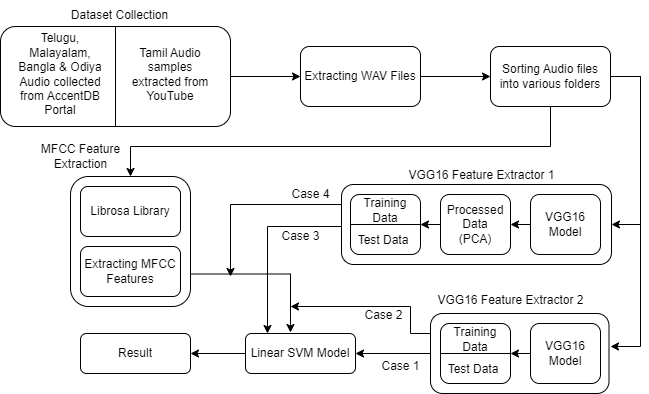
\includegraphics[scale=0.52]{DSA Arch.drawio.png}}
	\caption{Architecture for Accent classification model}
	\label{model-dsa}
\end{figure}

\subsection{About the dataset}\label{subsec1}
AccentDB is used as the main dataset for this scenario as there aren’t many audio datasets available which solely focus on Indian accent classification. The AccentDB dataset consists of two variants: Core and Extended. The Core type consists of WAV files which have 4 types of Indian accents: Telugu, Malayalam, Bangla and Odiya, while the extended type consists of 5 English accents in addition to
4 Indian accents. Since the focus is on classifying the Indian accents alone, the Core type of dataset is taken which is around 2.8GB in size (compressed) and has 6500 WAV files in it. Each file in the dataset is of 5 seconds length and consists
of 2 speakers in each accent folder. For the Tamil accent, manual scraping of the data from YouTube videos is done and stored in a folder with each WAV file having 5 second delay. All WAV audio files have 44100 Hz as sample rate which is
of high quality.

\subsection{Tools used}\label{subsec2}
The tools used in the proposed work are mentioned below:
\begin{itemize}
    \item Language:
    \begin{itemize}
        \item Python
    \end{itemize}
    \item Frameworks
    \begin{itemize}
        \item Tensorflow
        \item Keras
        \item Flask
    \end{itemize}
    \item Platform
    \begin{itemize}
        \item Google Colab
    \end{itemize}
    \item Audio Visualization and Analysis
    \begin{itemize}
        \item Librosa
    \end{itemize}
    \item Audio Extraction and Splitting (for external sources)
    \begin{itemize}
        \item Wondershare Filmora 11 
    \end{itemize}
    \item Dataset Downloader
    \begin{itemize}
        \item GDown library
    \end{itemize}
\end{itemize}

\section{Experimental Analysis}\label{sec4}
For the experiment, Python is used mainly for data pre-
processing, feature extraction and model training. For deployment, Flask is used to create a website where people can
upload their audio files which in turn would return the accent
as the result. In this section, the major parts of the experiment
work are described. The implementation is done using Google
Colab with GPU as hardware accelerator.

\subsection{Dataset collection}
Collecting data is the first and foremost step in the machine learning process. 
To extract the dataset from Google Cloud (both AccentDB and Custom data) in which the WAV files are stored, GDown library is used present in Python to download the tar files. After that, the tar file is extracted and the WAV files are obtained.


\subsection{Data Sorting}
After obtaining the WAV files, the files are stored on
separate folders which represent the particular class. In this
case, it’s the Indian languages. Since the file names are known
in this case, it’s easy to sort them into folders with the language
as the respective folder name. After sorting the WAV data, they
are sent to convert them as Waveform images.

\subsection{Waveform Images}
From the WAV data sorted, they are made to pass through
a function which will convert the amplitude values to image
format. This is done in order for VGG16 model to easily
segregate the features present in the waveform image of the
audio file.
The function is applied on a group of audio files instead
of every file in the dataset. This is done to reduce the load of the system as the system gets to peak RAM limit when
made to convert images from 6500 WAV files. So from every
language, 200-300 audio files are taken and they are made to
convert into images. These images are then sent to VGG16
model for extracting relevant features.

\begin{figure}[htbp]
	\centerline{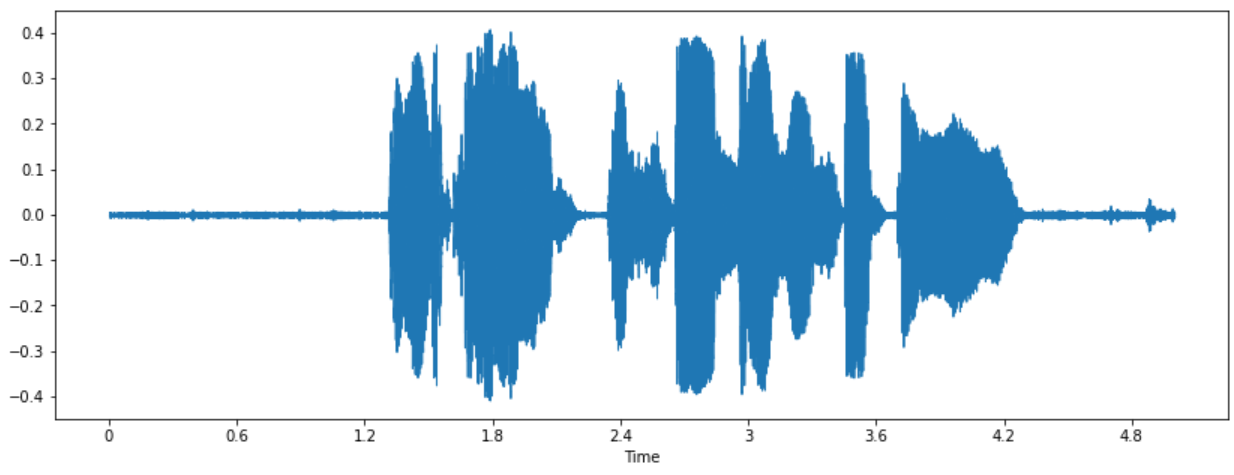
\includegraphics[scale=0.5]{wave-aud.png}}
	\caption{Waveplot image of a telugu WAV audio file}
	\label{wave-1}
\end{figure} 

\subsection{VGG16 model}
The VGG16 model is a Convolution Neural Network model created in 2014 to solve the Imagenet challenge.
When compared to the GoogLeNet architecture, the model performed well during the challenge.
However, the model is slow in terms of training speed and large in size, making it only suitable for certain applications. The architecture is shown in Fig. \ref{vgg16}

The pre-trained variant of VGG16 from Tensorflow is taken
for the implementation as the main objective is to extract
relevant features from the waveform images. The features
extracted are then stored on a list which will be later converted
to dataframe for further processing.

\begin{figure}[htbp]
	\centerline{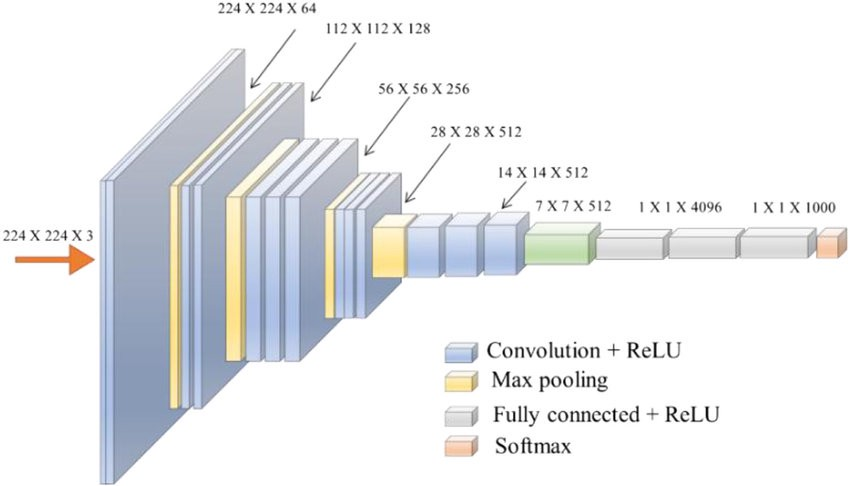
\includegraphics[scale=0.3]{vgg16.jpg}}
	\caption{VGG16 model \cite{b22}}
	\label{vgg16}
\end{figure}

There are many other CNN architectures available such as AlexNet, GoogleNet, ResNet-50, Inception-ResNet-v2 in which all of them are pre-trained. Except AlexNet, other models such as GoogleNet, ResNet are deep networks which are suitable only for training larger datasets. For smaller datasets, there is a risk of overfitting. So, a suitable network has to be chosen in this case. Compared with AlexNet, VGG16 has lower error rate and 16 layers; also VGG16 isn't as deep as compared with other networks, which makes it suitable to take for the proposed work though it has a large number of parameters. The comparison table is given in Table \ref{comp-1} for clarity. 

\begin{table*}[!htp]
	\caption{Comparision of CNN architectures}
	\begin{center}
		\resizebox{\textwidth}{!}{
		\begin{tabular}{p{4cm}p{2cm}p{2cm}p{3cm}p{2cm}p{1cm}}
			\cline{1-6}
			\textbf{\textit{CNN Architecture}}& \textbf{\textit{Year}} &
			\textbf{\textit{Number of Layers}} & \textbf{\textit{Number of Parameters}} & \textbf{\textit{Error Rate}} & 
			\textbf{\textit{Type}}\\
			\hline
			VGG16 & 2014 & 16 & 138M & 7.3\% & Deep \\
			\hline
			AlexNet & 2012 & 16 & 61M & 15.3\% & Shallow \\
			\hline
			GoogleNet & 2014 & 22 & 62.3M & 7.3\% & Deep \\
			\hline
			ResNet-50 & 2015 & 50 & 23M & 3.6\% & Deep \\
			\hline
			Inception-ResNet-v2 & 2016 & 164 & 56M & 4.9\% & Deep \\
			\hline
			Inception-v4 & 2016 & 22 & 43M & 5.0\% & Deep \\
			\hline
		\end{tabular}
	}
		\label{comp-1}
	\end{center}
\end{table*}

\subsection{MFCC features}
Mel Frequency Cepstral Coefficients (MFCCs) are a characteristic that is commonly employed in artificial speech and speaker recognition.
Prior to the introduction of MFCCs, the main feature type for automated speech recognition (ASR) was linear prediction coefficients (LPCs) and linear prediction cepstral coefficients (LPCCs), particularly used with HMM classifiers. 

To obtain the MFCC features, the basic algorithm is followed
below:\\
• The audio is divided into 20-40ms frames (25ms is
preferred). Then the frames are passed through a filter.\\
• The frames are made to pass through a function
which applies Fast Fourier Transform to convert them
from time domain to frequency domain.\\
• After conversion, the Mel scale is applied on the filters
to get a smooth spectrum which also reduces the size of
features.\\
• Finally, a discrete cosine transform is applied and the
respective coefficients are plotted.\\
To obtain the MFCC features from the WAV audio, Librosa
is used, which is a Python library made for music and
audio analysis. In this implementation, 40 MFCC features are
obtained from each audio and the features are stored in the
list (same as previous method) and then later converted into
dataframe for further processing.

The sample plot for MFCC is shown in Fig. \ref{mfcc}

\begin{figure}[htbp]
	\centerline{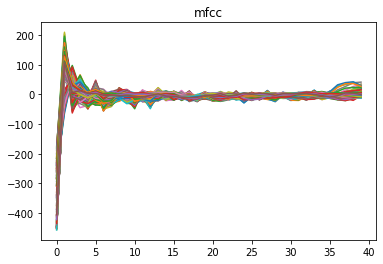
\includegraphics[scale=0.5]{mfcc.png}}
	\caption{Sample plot of MFCC for a WAV file}
	\label{mfcc}
\end{figure}

\subsection{LinearSVC model}
Support vector machines (SVMs) are supervised learning algorithms used for classification, regression, and outlier detection.
However, it is most often used for classification.
It operates on the principle of constructing a hyperplane that can segregate the majority of the points on the graph according to their class.

Here, LinearSVC (SVM with Linear Kernel) model is used with the help of scikit-learn module, and the model is trained using the training data generated in the previous stage.
As it is a classification model, the accuracy of the model with respect to testing data is calculated using the accuracy score. The architecture is shown in Fig. \ref{svm}

\begin{figure}[htbp]
	\centerline{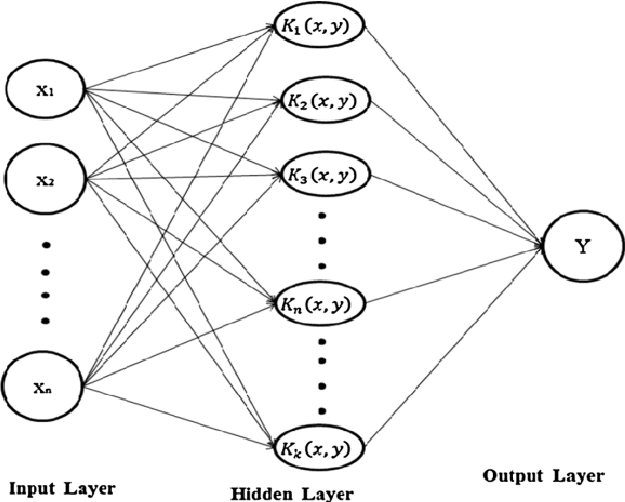
\includegraphics[scale=0.3]{dd.png}}
	\caption{SVM model \cite{b23}}
	\label{svm}
\end{figure}

\subsection{Data processing and training}
The lists created to store extracted features of audio via
VGG16 and MFCC features is then converted to data frames
via Pandas library. As the VGG16 feature vector is of huge
size for one audio (nearly 25088 features in total for 5 seconds), Principal Component Analysis method is
applied on every feature vector to reduce the overall feature
size to 40 in the data frame.
Then, the converted data frame is concatenated with the
MFCC feature data frame and the respective classes are labeled
manually in a list which ends the step. This processed dataset
is now sent for train-test split which is done in (75,25) method.
The obtained training and testing data is sent to LinearSVC
Model.

\subsection{Testing phase}
In this phase, first the model is made to be tested with the testing data
split earlier during the testing phase. The overall accuracy of the model is recorded with different kinds of features and required tweaks are done in order to improve the accuracy rate. Finally, the model is tested with real audio datasets which are obtained from random videos available in YouTube. Before giving the data, the audio data is made to convert to WAV format with 5 second slice format. Finally the data is made to pass into the model. The model was able to predict the target language provided that the audio is free of background noise such that the features can be captured easily. 

\subsection{Deployment}
For the deployment phase, the Flask library is used to
create a web app in which users can send the audio data and
view the accent type as the result. For saving VGG16 model
parameters, the model is made to export to HDF5 format while
the LinearSVC model parameters is exported with the help of
pickle library in python. After importing the parameters, the
Flask app is created and the model works pretty well along
with the web app. The sample app image is shown in Fig. \ref{app-1}

\begin{figure}[htbp]
	\centerline{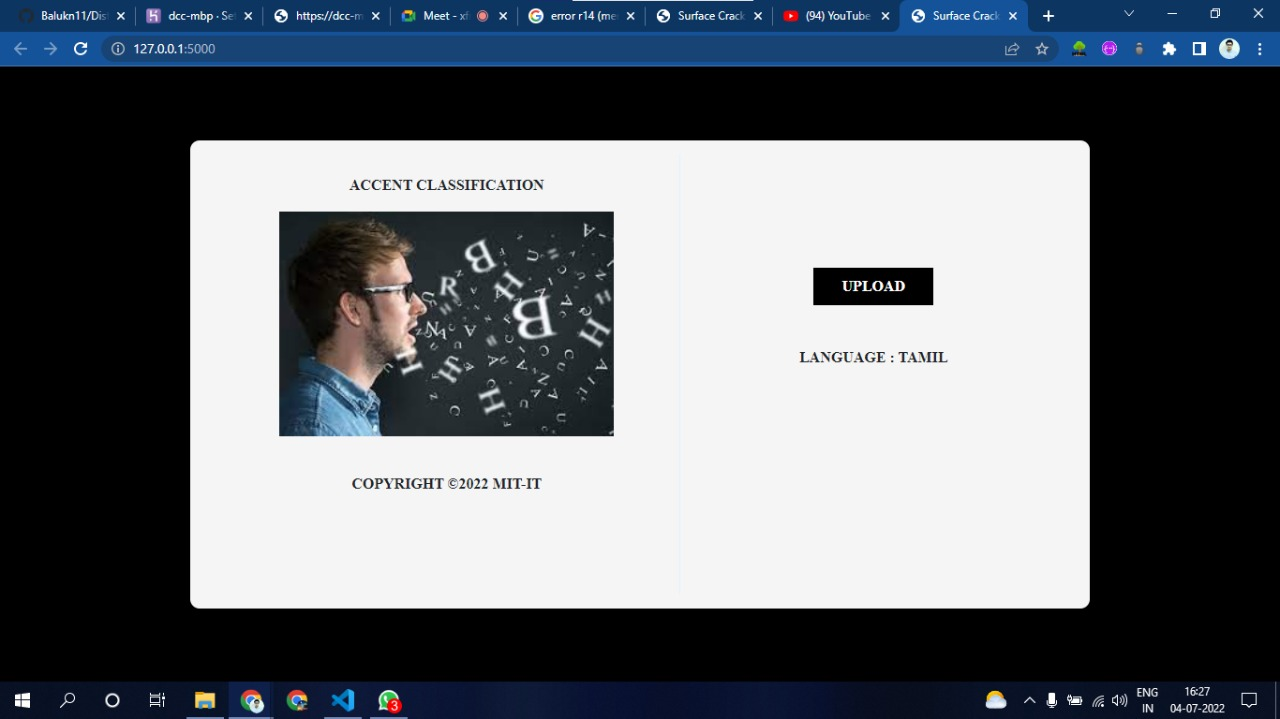
\includegraphics[scale=0.25]{app-1.jpg}}
	\caption{Result of model in Flask application}
	\label{app-1}
\end{figure}

\section{Output and End product}
Following the creation of the classification model and the web app, the models are tested with various data and it handles pretty well provided that the accents are within the class range. Since the focus isn’t on native accents, classification on non-native English Indian accents alone is made as the objective of the experiment. Even with real time data, the models classified the audio data with good accuracy. The accuracies of the models are recorded for 2 epochs and from them, the accuracy of the reduced VGG16 and MFCC features recorded the highest. The comparison table is also made in Table \ref{compare}

\begin{table}[!htbp]
\begin{center}
\caption{Accuracies of the features taken}\label{compare}%
\begin{tabular}{@{}lll@{}}
\toprule
Features taken & Accuracy (in percent) & Number of features taken\\
\midrule
Unreduced VGG16 & 86.46 & 25088 \\
Unreduced VGG16 and MFCC & 96.46 & 25128  \\
Reduced VGG16 & 71.46 & 40 \\
Reduced VGG16 and MFCC & 98.46 & 80 \\
\botrule
\end{tabular}
\end{center}
\end{table}

The final feature was finalized based on the accuracy patterns. Such that in order to find out the best fitting model a comparative analysis between four different approaches was carried out. First, the pre-trained model VGG16 was used as a feature extractor to get the features of the audio samples such as time with respect to audio. The number of features obtained from this model is 25088. All these features were fed into the SVM classifier model and this yielded an accuracy of 86.4\%. Secondly,  the previously obtained VGG16 features were combined with the Mel Frequency Cepstral Coefficient (MFCC) features and which collectively produced 25128 features. When these many features were trained using the SVM model and yielded 96.46\% of accuracy. The third observation is that, the features obtained from the first method were reduced to 40 features using Principal Component Analysis. This was done in order to cut down the curse of dimensionality issue, but this model yielded the lowest accuracy of 71.46\% percentage when compared with other approaches. The final method was conducted with the addition of reduced VGG16 features and MFCC, it totals up to 80 features. When these features were fed into the SVM model, it gave a maximum accuracy of 98.46\%. From these observations, the model having the maximum accuracy can be used to categorize the audio files of respective accents.

\section{Conclusion}
The VGG16-SVC model is developed such that it classifies the five native indian languages spoken in English. The features were extracted using the WAVfile package from scipy. Such that the amplitude and time at each frame are returned from the function and are made to visualize as wave plots. These images are stored and given as input to the VGG16 pre-trained model and the features are extracted accordingly. The acquired features are used as the inputs along with MFCC Features to the Support Vector Machine Classifier and the model is trained. When the trained model was validated, it attained an accuracy of about 98.46\%. This model would be useful to classify the Native languages such as Tamil, Malayalam, Odia, Telugu and Bangla. The number of data samples for each class can be increased and few more native languages can be added and classified. These may be considered as future works accordingly. \\

\noindent \textbf{Conflict of Interest:}

On behalf of all authors, the corresponding author states that there is no conflict of interest.
%\bibliography{sn-bibliography}
%% if required, the content of .bbl file can be included here once bbl is generated
%%\input sn-article.bbl
\newpage

\begin{thebibliography}{9}

\bibitem{b1}Tarun, M., Israr, A., Gajwal, D. (2022). ANALYSIS OF THE FACTORS INFLUENCE INDIAN ENGLISH ACCENTS, AND HOW PRONUNCIATION AND ARTICULATION FILL THE ACCENT GAP. EPRA International Journal of Environmental Economics, Commerce and Educational Management (ECEM), 9(4), 43–49.
\bibitem{b2} Mridha, M., Ohi, A., Hamid, M., Monowar, M. (2022). A study on the challenges and opportunities of speech recognition for Bengali language. Artificial Intelligence Review, 55(4), 3431–3455.
\bibitem{b3} Caballero, M., Moreno, A., Nogueiras, A. (2006). Multidialectal acoustic modeling: A comparative study. In Multilingual Speech and Language Processing.
\bibitem{b4} Suman, S., Sahoo, K., Das, C., Jhanjhi, N., Mitra, A. (2022). Visualization of Audio Files Using Librosa. In Proceedings of 2nd International Conference on Mathematical Modeling and Computational Science (pp. 409–418).
\bibitem{b5} Bodine, J., Hochbaum, D. (2022). A Better Decision Tree: The Max-Cut Decision Tree with Modified PCA Improves Accuracy and Running Time. SN Computer Science, 3(4), 1–18.
\bibitem{b6} Deshpande, Shamalee, Sharat Chikkerur, and Venu Govindaraju. "Accent classification in speech." Fourth IEEE Workshop on Automatic Identification Advanced Technologies (AutoID'05). IEEE, 2005.
\bibitem{b7} Upadhyay, R., Lui, S. (2018). Foreign English accent classification using deep belief networks. In 2018 IEEE 12th international conference on semantic computing (ICSC) (pp. 290–293).
\bibitem{b8} Ahmed, A., Tangri, P., Panda, A., Ramani, D., Karmakar, S. (2019). Vfnet: A convolutional architecture for accent classification. In 2019 IEEE 16th India Council International Conference (INDICON) (pp. 1–4).
\bibitem{b9} Guntur, R., Ramakrishnan, K., Mittal, V. (2022). Foreign Accent Recognition Using a Combination of Native and Non-native Speech. In Intelligent Sustainable Systems (pp. 713–721). Springer.
\bibitem{b10} Honnavalli, D., Shylaja, S. (2021). Supervised Machine Learning Model for Accent Recognition in English Speech Using Sequential MFCC Features. In Advances in Artificial Intelligence and Data Engineering (pp. 55–66). Springer.
\bibitem{b11} Guntur, R., Ramakrishnan, K., Vinay Kumar, M. (2022). An Automated Classification System Based on Regional Accent. Circuits, Systems, and Signal Processing, 41(6), 3487–3507.
\bibitem{b12} Krishna, G., Krishnan, R., Mittal, V. (2020). A system for automatic regional accent classification. In 2020 IEEE 17th India Council International Conference (INDICON) (pp. 1–5).
\bibitem{b13} Parikh, P., Velhal, K., Potdar, S., Sikligar, A., Karani, R. (2020). English language accent classification and conversion using machine learning. In Proceedings of the International Conference on Innovative Computing \& Communications (ICICC).
\bibitem{b14} Purwar, A., Sharma, H., Sharma, Y., Gupta, H., Kaur, A. (2022). Accent classification using Machine learning and Deep Learning Models. In 2022 1st International Conference on Informatics (ICI) (pp. 13–18).
\bibitem{b15} Duduka, S., Jain, H., Jain, V., Prabhu, H., Chawan, P. (2020). Accent Classification using Machine Learning. International Research Journal of Engineering and Technology (IRJET), 7(11), 638–641.
\bibitem{b16} Pedersen, C., Diederich, J. (2007). Accent classification using support vector machines. In 6th IEEE/ACIS International Conference on Computer and Information Science (ICIS 2007) (pp. 444–449).
\bibitem{b17} Badhon, S., Rahaman, H., Rupon, F., Abujar, S. (2021). Bengali accent classification from speech using different machine learning and deep learning techniques. In Soft Computing Techniques and Applications (pp. 503–513). Springer.
\bibitem{b18} Mannepalli, K., Sastry, P., Suman, M. (2016). MFCC-GMM based accent recognition system for Telugu speech signals. International Journal of Speech Technology, 19(1), 87–93.
\bibitem{b19} Duduka, S., Jain, H., Jain, H., Chawan, P. (2021). A Neural Network Approach to Accent Classification. International Research Journal of Engineering and Technology (IRJET), 8(03), 1175–1177.
\bibitem{b20} Hossain, P., Chakrabarty, A., Kim, K., Piran, M. (2022). Multi-Label Extreme Learning Machine (MLELMs) for Bangla Regional Speech Recognition. Applied Sciences, 12(11), 5463.
\bibitem{b21} Ahamad, A., Anand, A., Bhargava, P. (2020). Accentdb: A database of non-native english accents to assist neural speech recognition. arXiv preprint arXiv:2005.07973.
\bibitem{b22} Althubiti, S., Alenezi, F., Shitharth, S., Reddy, C., and others (2022). Circuit Manufacturing Defect Detection Using VGG16 Convolutional Neural Networks. Wireless Communications and Mobile Computing, 2022.
\bibitem{b23} Harini, V., Bhanumathi, V. (2016). Automatic cataract classification system. In 2016 international conference on communication and signal processing (ICCSP) (pp. 0815–0819).
\end{thebibliography}

%% Default %%
%%\input sn-sample-bib.tex%

\end{document}
